% THIS IS SIGPROC-SP.TEX - VERSION 3.1
% WORKS WITH V3.2SP OF ACM_PROC_ARTICLE-SP.CLS
% APRIL 2009

\documentclass{acm_proc_article-sp}

\usepackage[slovene,english]{babel}
\usepackage[utf8]{inputenc}

\begin{document}

\title{FbHash: A New Similarity Hashing Scheme for Digital Forensics}
%\subtitle{[Extended Abstract]
%\titlenote{A full version of this paper is available as
%\textit{Author's Guide to Preparing ACM SIG Proceedings Using
%\LaTeX$2_\epsilon$\ and BibTeX} at
%\texttt{www.acm.org/eaddress.htm}}}

\numberofauthors{3} 
\author{
\alignauthor
Timotej Knez \\
63..%\titlenote{Dr.~Trovato insisted his name be first.}\\
%       \affaddr{Institute for Clarity in Documentation}\\
%       \affaddr{1932 Wallamaloo Lane}\\
%       \affaddr{Wallamaloo, New Zealand}\\
%       \email{trovato@corporation.com}
% 2nd. author
\alignauthor
Sebastian Mežnar\\
27192031 %\titlenote{The secretary disavows
%any knowledge of this author's actions.}\\
%       \affaddr{Institute for Clarity in Documentation}\\
%       \affaddr{P.O. Box 1212}\\
%       \affaddr{Dublin, Ohio 43017-6221}\\
%       \email{webmaster@marysville-ohio.com}
% 3rd. author
\alignauthor 
Jasmina Pegan \\
63170423%\titlenote{This author is the
%one who did all the really hard work.}\\
%       \affaddr{The Th{\o}rv{\"a}ld Group}\\
%       \affaddr{1 Th{\o}rv{\"a}ld Circle}\\
%       \affaddr{Hekla, Iceland}\\
%       \email{larst@affiliation.org}
}

\date{18 april 2020}

\maketitle
\begin{abstract}
%TODO
nek povzetek
\end{abstract}

\category{E.3}{Data encryption}{}

\terms{Hashing}

\keywords{Data fingerprinting, Similarity digests, Fuzzy hashing, TF-IDF, Cosine-similarity} 

\section{Uvod}
Živimo v obdobju shranjevanja ogromnih količin podatkov. Pri forenzičnih preiskavah se pogosto zgodi, da je pridobljenih datotek preveč za ročno pregledovanje. Digitalni forenziki se tako soočijo s problemom avtomatizacije preiskave datotek. Možna rešitev so algoritmi, kot so \texttt{ssdeep}, \texttt{sdhash} in \texttt{FbHash}, ki poskusijo filtrirati vnaprej znane "slabe" oziroma "dobre" datoteke. Ti algoritmi (angl. \emph{Approximate Matching algorithms}) ugotavljajo delež ujemanja datotek s pomočjo (nekriptografskih) zgoščevalnih funkcij. Algoritma \texttt{ssdeep} in \texttt{sdhash} lahko preslepi aktivni napadalec, ki pametno napravi majhne spremembe na določenih mestih datoteke. Učinkovitega napada na algoritem \texttt{fbhash} ne poznamo.\cite{fbhash}
%TODO
% nekej o FbHash-B in S in primeri tipa datotek
% še kaj o naši implementaciji, poskusih, rezultatih

V 2. poglavju predstavimo predhodnike algoritma \texttt{FbHash}. V 3. poglavju podrobneje predstavimo algoritem \texttt{FbHash} in našo implementacijo. V 4. poglavju opišemo izvedene eksperimente in  v 5. poglavju opišemo rezultate. V 6. poglavju povzamemo narejeno delo in rezultate.

\section{Sorodna dela}
Prvi algoritem, namenjen iskanju približnih ujemanj, je bil objavljen leta 2002 pod imenom \texttt{dcfldd}. Ta algoritem je razvil N. Harbour kot izboljšano verzijo ukaza \texttt{dd}\cite{dcfldd}. Izboljšana različica tega algoritma je \texttt{ssdeep}. Pomembnejša predhodnika algoritma \texttt{FbHash} sta tudi \texttt{MRSH-v2} in \texttt{mvHash-B}. Obstaja še \texttt{bbhash}, ki pa je časovno potraten in ga ne bomo podrobneje opisali.

\subsection{ssdeep}
Algoritem \texttt{ssdeep} je implementacija kontekstno sprožene kosovno zgoščevalne funkcije (angl. \emph{Context Triggered Piecewise Hash}, CTPH), ki jo je predstavil J. Kornblum septembra 2006 v članku~\cite{kornblum:ctph}. Algoritem temelji na detektorju neeželene elektronske pošte \texttt{spamsum}, ki lahko zazna sporočila, ki so podobna znanim neželenim sporočilom.

CTPH uporablja zgoščevanje po kosih (angl. \emph{piecewise hashing}), kar pomeni, da se zgoščena vrednost izračuna na posameznih kosih fiksne dolžine. Za razliko od \texttt{dcfldd}, algoritem CTPH uporabi poljubno zgoščevalno funkcijo.

Drugi princip, ki ga uporablja CTPH, je zgoščevalna funkcija z drsečim oknom (angl. \emph{rolling hash}), ki preslika zadnjih $k$ zlogov (bajtov) v psevdonaključno vrednost. Vsakega naslednika je tako možno hitro izračunati iz predhodno izračunane vrednosti. Pri tem je uporabljena zgoščevalna funkcija \texttt{FNV}.

Postopek CTPH se začne z izračunom zgoščenih vrednosti z drsečim oknom. Ob določeni sprožilni zgoščeni vrednosti (angl. \emph{trigger value}) se vzporedno s tem sproži še algoritem zgoščevanja po kosih. Ob ponovni pojavitvi sprožilne vrednosti se dotlej zbrane vrednosti druge zgoščevalne funkcije zapišejo v končni prstni odtis.
Tako se ob lokalni spremembi v datoteki sprememba pozna le lokalno tudi v prstnem odtisu.

Sledi primerjava prstnih odtisov datotek, ki temelji na uteženi Levenstheinovi razdalji (angl. \emph{edit distance}), ki je nato še skalirana in obrnjena, da predstavlja $0$ povsem različna prstna odtisa.

Algoritem \texttt{ssdeep}, ki je implementacija CTPH, se izkaže pri primerjavi podobnih besedilnih datotek in dokumentov~\cite{kornblum:ctph}. Po drugi strani pa lahko aktivni napadalec popravi "slabe" datoteke na tak način, da se izognejo črni listi~\cite{fbhash}. Ker je prstni odtis fiksne dolžine, je algoritem primeren le za relativno majhne datoteke podobnih velikosti.

\subsection{sdhash}
Algoritem \texttt{sdhash} je opisal V. Roussev januarja 2010 v članku~\cite{roussev:sdhash}. Glavna prednost tega algoritma pred predhodnimi je, da izbere statistično manj verjetne dele datotek kot izhodišče za računanje prstnega odtisa.

Postopek se začne z iskanjem statistično najmanj verjetnih delov datoteke. Izračuna se entropija skupin po $k$ zlogov datoteke. Nato se izračuna rank vsake skupine glede na $n$ sosednjih skupin. Izbrane so skupine, ki imajo rank večji ali enak postavljeni meji.

Sledi filtriranje skupin $k$ zlogov, ki niso bistvene, povzročajo pa lažno pozitivne rezultate. Ocenili so, da je dobro zavreči skupine z oceno entropije pod $100$ ali nad $990$, ker so takšne skupine pogoste v datotekah tipa JPEG.

Nato se generira prstni odtis datoteke kot zaporedje Bloomovih filtrov, ki so verjetnostne strukture, uporabljene za prostorsko učinkovito predstavitev množic. Algoritem \texttt{sdhash} preveri za vsako izbrano skupino $k$ zlogov, ali je že v množici, predstavljeni z Bloomovimi filtri. Če skupine ni v množici, jo algoritem doda.

Nazadnje algoritem primerja prstne odtise datotek, torej zaporedje Bloomovih filtrov. Za vsak filter, ki predstavlja prvo datoteko, se izračuna maksimalna ocena podobnosti s filtri, ki predstavljajo drugo datoteko. Rezultat je povprečje tako pridobljenih ocen podobnosti.

Algoritem \texttt{sdhash} doseže boljša priklic in preciznost kot \texttt{ssdeep}~\cite{fbhash}. A tudi ta algoritem ima več pomanjkljivosti: nekaterih datoteke ne more primerjati, primerjava datoteke same s seboj lahko vrne oceno med $50$ in $100$ ter prvih $15$ zlogov sploh ne vpliva na končni prstni odtis. Poleg naštetega aktivni napadalec lahko spremeni "slabe" datoteke na tak način, da se izognejo črni listi oziroma "dobre" datoteke tako, da se obdržijo na beli listi~\cite{breitinge2012security}.

\subsection{MRSH-v2}
Oktobra 2012 sta F. Breitinger in H. Baier predstavila algoritem \texttt{MRSH-v2}~\cite{mrsh-v2}, ki se opira na predhodno razvit algoritem \texttt{MRSH} (angl. \emph{multi-resolution similarity hashing}), ta pa temelji na algoritmu \texttt{ssdeep}. 

Algoritem \texttt{MRSH} ima določene sprožilne točke $-1 mod b$, kjer $b$ pomeni povprečno velikost bloka. Namesto zgoščevalne funkcije z drsečim oknom uporabi polinomsko zgoščevalno funkcijo \texttt{djb2}, kot primitiv pa \texttt{MD5}. Namesto konkatenacije zgoščenih vrednosti \texttt{MRSH} kot prstni odtis uporabi seznam Bloomovih filtrov. 

Algoritem \texttt{MRSH-v2} ponovno uporabi zgoščevalno funkcijo z drsečim oknom, kot \texttt{ssdeep}, namesto \texttt{FNV} pa uporabi funkcijo zgoščevanja \texttt{MD5}. Za večjo hitrost in v izogib napadu z dodajanjem sprožilnih točk je dodana tudi spodnja meja za velikost skupin zlogov $\frac{b}{4}$. 

Algoritem \texttt{MRSH-v2} je po~\cite{mrsh-v2} časovno učinkovitejši od predhodnih algoritmov. Vključuje način za odkrivanje fragmentov in način za odkrivanje podobnih datotek. Po analizi leta 2014~\cite{breitinger2014}, ki primerja \texttt{ssdeep}, \texttt{sdhash} in \texttt{MRSH-v2}, se v povprečju najbolje obnese \texttt{sdhash}, \texttt{ssdeep} in \texttt{sdhash} izkazujeta dobro preciznost, vsi trije algoritmi pa imajo relativno slab priklic.

\subsection{mvHash-B}
Marca 2013 so F. Breitinger in sod. predstavili algoritem \texttt{mvHash-B}~\cite{mvhash-b}. Ideja algoritma je, da majhne lokalne spremembe ne spremenijo končnega rezultata. 

V prvem koraku se izvede večinsko glasovanje po bitih z nastavljivo mejo $t$. Vsakih $k$ zlogov se tako preslika v ničle, če je število enic v zaporedju bitov manjše od $t$, sicer pa v enice.

Nato se zaporedje bitov zapiše na bolj kompakten način -- enake zaporedne bite nadomestimo z dolžino takega niza. Če se zaporedje bitov ne začne z nekaj ničlami, bo prvo število v seznamu 0. Dobimo kodirano zaporedje dolžin nizov.

Kodirano zaporedje se razdeli v prekrivajoče se skupine fiksne dolžine. Te skupine so dodane v Bloomov filter.
Nazadnje se primerja Bloomove filtre s pomočjo Hammingove razdalje, ocene pa se povpreči in odšteje od $100$. 

Algoritem \texttt{mvHash-B} naj bi bil hiter skoraj kot \texttt{SHA-1}, torej blizu zgornje meje učinkovitosti~\cite{mvhash-b}. Vendar tudi ta algoritem ni varen pred aktivnim napadalcem, saj je možno popraviti "slabo" datoteko tako, da se izogne črni listi~\cite{chang2016security}.

\section{Algoritem}

Avtorji v članku \cite{fbhash} predstavijo algoritem \texttt{FbHash-B}, ki je namenjen nestisnjenim (ang. uncompressed) in \texttt{FbHash-S}, ki je namenjen stisnjenim (ang. compressed) datotekam. Iskanje želenih datotek poteka na sledeč način. Najprej datoteke, ki jih želimo preveriti zgostimo s pomočjo ustreznega algoritma glede na njihov tip in tako dobim bazo podatkov. Nato zgostimo še ciljne datoteke in jih primerjamo z datotekami iz baze podatkov. Tako lahko datoteke, ki imajo s ciljnimi dovolj podobnosti zavržemo (ang. blacklist) oziroma dodamo med iskane (ang. whitelist).

\subsection{FbHash-B}

\texttt{FbHash-B} je bolj primeren datotekam, ki niso stisnjene. V opisu algoritma bomo za boljšo preglednost uporabili sledečo notacijo:
% TODO: mogoce zmanjsaj prostor med dvema tockama
\begin{itemize}
  \item Del datoteke: niz k zaporednih bajtov. 
  \item $ch_{i}^D$: del datoteke D, ki se začne na i-tem bajtu.
  \item Frekvenca dela oziroma $chf_{ch_i}^D$: število pojavitev dela $ch_i$ v datoteki D.
  \item Dokumentna frekvenca dela oziroma $df_{ch}$: število dokumentov, ki vsebujejo del datoteke $ch$.
  \item $N$: število datotek v bazi podatkov.
  \item $RollingHash(ch_i)$: vrednost rekurzivne zgoščevalne funkcije imenovane rolling hash na delu besedila $ch_i$
  \item $chw_{ch_i}$: utež dela besedila $ch_i$
  \item $docw_{ch_i}$: dokumentna utež dela besedila $ch_i$
  \item $W_{ch_i}^D$: ocena dela besedila $ch_i$ v dokumentu D
\end{itemize}

Algoritem je predstavljen v treh korakih. Prvi zavzema računanje frekvence delov datotek, drugi računanje dokumentnih uteži delov datotek in tretji računanje zgostitvenih uteži.

\subsubsection{Računanje frekvence delov datotek}

V tem koraku se izračunajo frekvence delov datotek in njihove uteži. Vsaka datoteka vsebuje $N_D - k$ delov datotek, kjer je $N_D$ dolžina datoteke D v bajtih in k parameter. Tako ima i-ti del datoteke D obliko $B_{i}^{D}B_{i+1}^{D}...B_{i+k-1}^{D} = ch_{i}^D$, kjer je $B_{j}^{D}$ j-ti bajt v datoteki D.

Najprej izračunamo $RollingHash(ch_{0}^D)$ s formulo \begin{displaymath} RollingHash(ch_{0}^D) = (B_{0}^{D}*a^{k-1} + B_{1}^{D}*a^{k-2} + ... + B_{k-1}^{D}*a^0)\, mod\, n \end{displaymath}, kjer so a, n in k parametri. Zaradi rekurzivne strukture funkcije $RollingHash$ lahko zgostitve preostalih delov izračunamo na sledeč način: \begin{displaymath} RollingHash(ch_{i+1}^D) = (a*RollingHash(ch_{i}^D)-B_{i}^{D}*a^{k}-B_{i+k}^D)\, mod\, n \end{displaymath}

Parametre a, k in n izberemo na sledeč način. Za a izberemo neko konstanto med 2 in 255. Če za zalogo vrednosti funkcije RollingHash vzamemo 64 bitna števila, lahko k izračunamo na sledeč način: \begin{displaymath}  B_{i}^{D}* a^{k-1} \leq 2^{64}-1\end{displaymath}. Ker je maksimalna vrednost bajta in parametra a enaka 255 dobimo neenačbo $255^k \leq 2^{64}-1$ iz česar sledi, da je k manjši ali enak 7. Tako za k izberemo 7. Če želimo zagotoviti, da ne pride do trkov med različnimi deli datotek, moramo za n izbrati prašteviko, ki je večje od $2^56=255*255^{k-1}$. 

Strukturo datoteke lahko tako predstavimo kot razpršeno tabelo, kjer je kjuč vrednost, ki jo dobimo s funkcijo $RollingHash$ na določenem delu datoteke, vrednost pa število pojavitev pripadajočega dela datoteke (oziroma vrednosti, ki smo jo dobili s funkcijo $RollingHash$).

Prvi korak zaključimo tako, da izračunamo uteži za dele besedila znotraj datoteke ($chw_{ch_i}$) s pomočjo ene izmed funkcij iz \ref{weight-functions}.

\subsubsection{Računanje dokumentnih uteži}

\subsubsection{Računanje zgostitvenih uteži}

\subsection{FbHash-S}

FbHash-S je bolj primeren za stisnjene datoteke tipa docx, pptx, pdf, zip, ...

\subsection{Primerjanje dokumentov}

\subsection{Uporabljene funkcije za uteževanje}
\label{weight-functions}

\section{Na\v{s}i eksperimenti (name in progress)}

\section{Rezultati}

\section{Zaklju\v{c}ek}

\section{Zahvala}
Mogoče zahvala avtorjem za narjeno delo al kej.

\bibliographystyle{abbrv}
\bibliography{sigproc}  % sigproc.bib is the name of the Bibliography in this case
% You must have a proper ".bib" file
%  and remember to run:
% latex bibtex latex latex
% to resolve all references

%%\balancecolumns
%\appendix
%%Appendix A

\balancecolumns
\end{document}

% Now, we'll enter an unnumbered equation:
%\begin{displaymath}\sum_{i=0}^{\infty} x + 1\end{displaymath}
%and follow it with another numbered equation:
%\begin{equation}\sum_{i=0}^{\infty}x_i=\int_{0}^{\pi+2} f\end{equation}
%just to demonstrate \LaTeX's able handling of numbering.

%To set a wider table, which takes up the whole width of the page's live area, use the environment \textbf{table*} to enclose the table's contents 

%\begin{table*}
%\centering
%\caption{Some Typical Commands}
%\begin{tabular}{|c|c|l|} \hline
%Command&A Number&Comments\\ \hline
%\texttt{{\char'134}alignauthor} & 100& Author alignment\\ \hline
%\texttt{{\char'134}numberofauthors}& 200& Author enumeration\\ \hline
%\texttt{{\char'134}table}& 300 & For tables\\ \hline
%\texttt{{\char'134}table*}& 400& For wider tables\\ \hline\end{tabular}
%\end{table*}
% end the environment with {table*}, NOTE not {table}!

%\begin{figure}
%\centering
%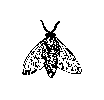
\epsfig{file=fly.eps}
%\caption{A sample black and white graphic (.eps format).}
%\end{figure}

%\begin{figure}
%\centering
%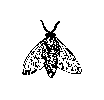
\epsfig{file=fly.eps, height=1in, width=1in}
%\caption{A sample black and white graphic (.eps format)
%that has been resized with the \texttt{epsfig} command.}
%\end{figure}

%As was the case with tables, you may want a figure that spans two columns. \textbf{figure*} to enclose the figure and its caption.

%\begin{figure*}
%\centering
%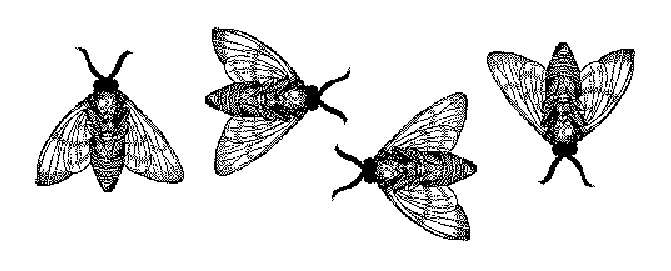
\epsfig{file=flies.eps}
%\caption{A sample black and white graphic (.eps format)
%that needs to span two columns of text.}
%\end{figure*}
%and don't forget to end the environment with
%{figure*}, not {figure}!

%This uses the \textbf{theorem} environment, created by
%the\linebreak\texttt{{\char'134}newtheorem} command:
%\newtheorem{theorem}{Theorem}
%\begin{theorem}
%Let $f$ be continuous on $[a,b]$.  If $G$ is
%an antiderivative for $f$ on $[a,b]$, then
%\begin{displaymath}\int^b_af(t)dt = G(b) - G(a).\end{displaymath}
%\end{theorem}

%The other uses the \textbf{definition} environment, created
%by the \texttt{{\char'134}newdef} command:
%\newdef{definition}{Definition}
%\begin{definition}
%If $z$ is irrational, then by $e^z$ we mean the
%unique number which has
%logarithm $z$: \begin{displaymath}{\log e^z = z}\end{displaymath}
%\end{definition}

%the \textbf{proof} environment.  Here
%is a example of its use:
%\begin{proof}
%Suppose on the contrary there exists a real number $L$ such that
%\begin{displaymath}
%\lim_{x\rightarrow\infty} \frac{f(x)}{g(x)} = L.
%\end{displaymath}
%Then
%\begin{displaymath}
%l=\lim_{x\rightarrow c} f(x)
%= \lim_{x\rightarrow c}
%\left[ g{x} \cdot \frac{f(x)}{g(x)} \right ]
%= \lim_{x\rightarrow c} g(x) \cdot \lim_{x\rightarrow c}
%\frac{f(x)}{g(x)} = 0\cdot L = 0,
%\end{displaymath}
%which contradicts our assumption that $l\neq 0$.
%\end{proof}